%!TEX root = ../thesis.tex

\chapter{Introduction}
\label{chap:i}

\section{Motivation}
\label{sec:motivation}

Constructing and maintaining an up-to-date graph-like road network on the national level has a range of firmly established uses. Owing to its structure, it can be used efficiently for modelling and simulation purposes, such as traffic flow simulations, passenger transport modelling, construction and upgrade impact modelling (to pinpoint optimal locations and types of investment), and traffic noise load modelling (\cite{bell_lida_1997, zhu_li_2007, zhang_2011, duran_santos_2014, peng_etal_2020}). It can also be used for navigation; a graph-like road network representation is at the heart of most road navigation services (\cite{yue_etal_2008}). Combined with other datasets, we can mention an even wider range of use cases: complemented by ecological statistics and models, it can offer insight into the impact of the presence of roads, and planned road construction on the flora and fauna in their vicinity.

Or to mention a different type of example, a digital road network may be used as a shared working space when aggregating geospatial data relating to road infrastructure from various sources. It makes it possible for geographical road locations, topographical relationships, and arbitrary semantic information to reside in the same network-type data model, making analysis techniques more straightforward, enforcing consistency and saving effort for data providers who would otherwise all need to maintain their own road models (\cite{ekpenyong_etal_2007}). This example is closely related to the ambitions of the provider of the Dutch digital road network that is the primary subject of this research.

One may remark that a two-dimensional representation with \textit{approximate} geographical locations may suffice for many of the purposes I listed as examples above, topology being the main concern in network analysis. For instance, \ac{gnss} navigation software often use snapping methods to ensure that the navigating vehicle always traverses the road graph – ensuring that navigation remains continuous even when positioning has poor accuracy (\cite{fouque_bonnifait_2008}). Traffic flow simulations are primarily concerned with traffic loads, road properties, and how roads are subdivided by intersections. \textit{Mostly}, they are not concerned with the exact geographical locations of roads – as long as the topology is relatively accurate, any geographical permutation of the network will yield largely invariant results (\cite{thomson_richardson_1995}).

However, some applications are concerned with the road network in the context of its surroundings, which makes the accuracy of its georeferencing important. Noise modelling is such an application, because it requires deriving the noise load affecting various objects in the vicinity of the the roads. This also involves considering objects that may impact the propagation of the noise, such as noise barriers, terrain, and buildings (\cite{ishiyama_etal_1991, bennett_1997, guarnaccia_quartieri_2012}).

A realistic noise propagation model mainly takes into account terrain, and the 3D geometry of the surrounding objects. However, the position of roads \textit{relative to the terrain} should also be taken into account. For instance, consider a hill with a building on one side and a road on the other, as shown in Figure \ref{fig:justification_illu}. The hill (representing the terrain) in this case acts as a noise barrier affecting the noise load received by the building. Unless the assumption holds that roads are always found \textit{exactly on} the terrain, this is not yet enough information to derive the noise load incident on the building. Roads may be elevated, sunken into the ground, or built in tunnels – meaning that the assumption does not always hold. For instance, if the road in my example was built on a bridge with a similar height as the hill, then the hill suppresses the road noise much less effectively, and "snapping" the road to the terrain by ignoring its elevation would yield incorrect noise modelling results. One way to handle such scenarios is to take into account the absolute elevation of the road surfaces, in other words to use a 3D road network.

\begin{figure}
    \centering
    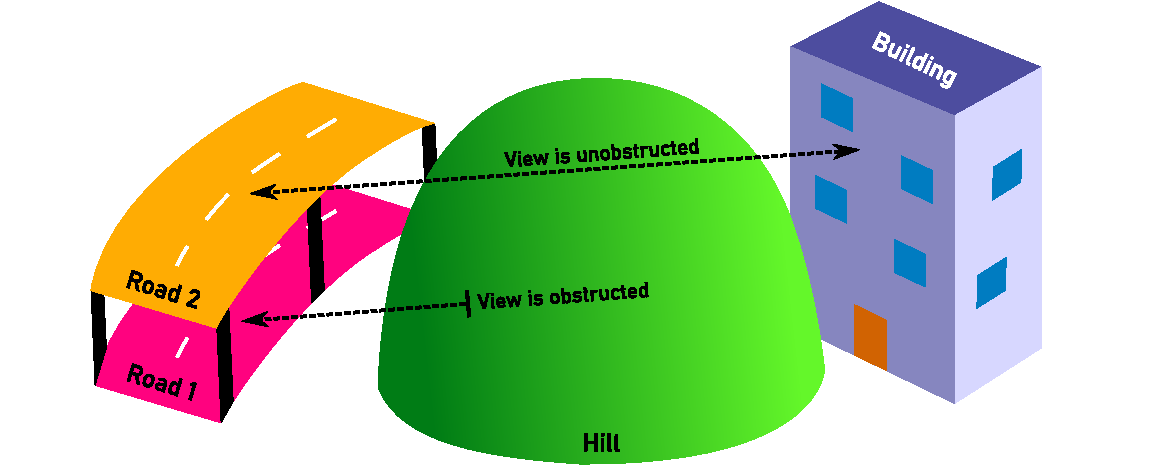
\includegraphics[width=\linewidth]{final_report/figs/justification_illu.pdf}
    \caption[Illustration of the 3D conversion justification]{This illustration shows a justification for the 3D conversion of digital road networks. Assuming that the roads always lie on the terrain (pink road) allows one to model the propagation of noise with the surrounding terrain and 3D objects taken into account. However, roads above or below the terrain will result in faults in the model. For instance, the noise from an arbitrary elevated version of this road (yellow road) would reach the building. "Snapping" it to the terrain suggests incorrectly that the hill blocks the noise.}
    \label{fig:justification_illu}
\end{figure}

2D-projected digital road models with mediocre accuracy have attracted great scientific and commercial attention since the advent of digital cartography and satellite navigation (\cite{taylor_etal_2001, fouque_bonnifait_2008, yue_etal_2008}). However, \textit{accurate 3D representations} are still atypical, owing to factors such as the increased cost of generation and maintenance, increased complexity of visualisation and analysis, and a lack of significant use cases (\cite{zhu_li_2007, wang_etal_2014}). As a result, 2D road models are common in terms of both public and private geospatial providers, whereas accurate 3D road models are rare in comparison.

When a use case arises and an accurate 3D model is needed, providers generally have two options: to produce a new model, or to enrich an existing 2D model with elevation data. The decision generally depends on the quality of the available 2D data set relative to the requirements for the 3D model, as well as that of the dataset(s) available as sources of elevation data, among other factors (\cite{zhu_li_2007, zhu_li_2008, wang_etal_2014}). In the geospatial field data acquisition is far more expensive than re-using existing datasets, especially openly available ones. As a result, many providers first attempt to find a way to convert their datasets into 3D using existing data in such a cost-effective manner.

\section{The NDW commission}
\label{sec:commission}

In certain projects the accuracy requirement and restrictions on the modelling procedure may be prescribed legally. Such is the case for the client of the present research, \ac{ndw} (National Road Traffic Data Portal), a division of \ac{rws} (Directorate-General for Public Works and Water Management). This Dutch government organisation is in the process of enriching their pre-existing open data 2D road model \ac{nwb} (National Road Database) with 3D data, to attain compliance with the new version of the Dutch noise legislation or \textit{geluidwetgeving}, coming into effect on the 1\textsuperscript{st} of January 2022. The new version of the legislation prescribes, among other things, a horizontal \textit{and vertical} accuracy of 20 centimetres for the road model underlying the noise simulations. Due to cost considerations and reasons related to \ac{ndw}’s data acquisition pipeline, the pre-existing 2D version of \ac{nwb} will be converted into a 3D dataset (dubbed \textit{3D-NWB}) primarily using open data geospatial datasets. They have produced a prototype implementation themselves, and subsequently contracted the consultant firm \ac{rhdhv} to create a commercial implementation based on their experience with the prototype. The development of this tool was concluded in December 2020, with a preliminary version of 3D-NWB already publicly available on their website in addition to the original 2D version.

Thus for \ac{ndw}, the next year will be about assessing the quality of their new product and improving it as they see necessary. In particular, they wish to assess how it fares in terms of the requirements set by law. This dissertation research attempts to contribute to this assessment by presenting an original system design and implementation that favours scientific correctness, and in which output accuracy can be qualitatively and quantitatively described. By comparing the results of the academic system design and implementation to the commercial one, it becomes possible to indirectly evaluate the commercial results' general quality and accuracy in an indirect manner. My work also explores various related topics that are not directly intended for this purpose, which I refer to as the solely academic aims of this project.

My research was carried out in consultation with the above parties. In fact, the stages leading up to the submission of my dissertation proposal involved thorough consultation with personnel both at \ac{ndw} and \ac{rhdhv} while the commercial implementation was still being developed, to ensure that my research fits well with \ac{ndw}'s plans and the commercial implementation.

\section{Field and relevance}
\label{sec:relevance}

For reasons that will later become clear (see Section \ref{sec:input}), I primarily focused on a Lidar point cloud and a 3D topographical line dataset as elevation sources. In both of these datasets, it is clearly evidenced that roads are occasionally in complex three-dimensional relationships with one another and with their environment. For instance, they cross above and below other roads and are also frequently occluded by other objects such as vegetation and buildings. Already in the planning phase of the project the question had arisen, how such real-world geometries should be dealt with in the conversion process – evidently they will require special treatment relative to well-exposed road surfaces. The answer to this question is closely linked with which field of the geosciences my project is positioned in.

The likely candidates in the context of digital road network modelling are \ac{gis} and geomatics (also called geoinformatics). It is thus worth discussing briefly how each typically treats 3D objects. One of the reasons why 2D road models are popular is that their geometry and network properties can be analysed using a multitude of well-proven \ac{gis} methods and software kits. However, in \ac{gis} models, even if elevation measurements exist, they are generally only present as an \textit{elevation attribute} (i.e. a semantic data field, like street names), because \ac{gis} geometrical models do not typically support true 3D operations. This is conceptually identical to projecting the geometries onto the horizontal plane. Geometric models that treat the vertical dimension explicitly are more common in geomatics; namely 2.5D and 3D models. While using 2.5D models restricts the types of physical entities that can be modelled, it also greatly simplifies certain types of analysis conceptually and computationally. This makes it ideal for working on similar scales to \ac{gis}; i.e. on the national scale for instance, as in this research.

While 2.5D modelling initially appears to be a good candidate for this project, we may observe that it is by definition unsuitable for handling the 3D relationships that roads have with each other and with their environment. However, much like how the concept of divide-and-conquer works in computer science, it possible decompose three-dimensional, geometrical problems into smaller sub-problems until they become natively compatible with 2.5D methods which are simpler to solve individually than the 3D problem as a whole. This research is positioned in the field of geomatics because my system design is specifically intended to explore how 2.5D methods can be applied in a way that enables the \textit{piecewise} modelling of a national road network. The divide-and-conqer concept is applied to decompose the road network into segments that can be individually, locally regarded as \textit{terrain} (i.e. a mathematical surface) and hence be modelled in 2.5D.

Geomatics is comprised of a wide range of disciplines, several of which are relevant to the present research. As I focused on 2.5D methods to a great extent, it overlaps with the geomatics field of \textit{digital terrain modelling} in terms of how it generates and stores the digital representations of roads, and as a consequence, the manner in which it derives elevations from them: using \textit{spatial interpolation}. As the overview of the methods in Section \ref{sec:methodsoverview} reveals, it also strongly overlaps with the geomatics discipline of \textit{feature extraction} (and to a lesser extent, \textit{photogrammetry}), because of the intermediate steps used by the pipeline to derive the 2.5D road surface models from our input datasets.

This is in line with my goal to study how a combination of mainly geomatics-based tools and methods can be used to accomplish the tasks required by \ac{ndw}, and to also assess their accuracy and suitability when used in this way. However, I also use \ac{gis} methods "under the hood" in all parts of the project – for instance, 2D geometry intersection tests, orientation tests and spatial queries are pervasive in the implementation, and are thus often mentioned in the detailed description of the processing steps found in Section \ref{sec:methods}. Furthermore, my research often touches on mathematics and statistics, for instance I use polynomial fitting and \ac{mle} throughout the implementation (as examples of the former) and metrics such as standard deviation and \ac{rmse} (as examples of the latter).

\section{Research questions}
\label{sec:rq}

My main research question is \textit{"How can we achieve a 3D conversion of the \ac{nwb} dataset using Dutch open geospatial data and a primarily 2.5D-based surface modelling methodology, while guaranteeing optimal and quantifiable accuracy and completeness?"}. It was distilled from the main areas of interest that we settled on during the preparatory stages of the project, while planning the project with my academic mentors, \ac{ndw}, and \ac{rhdhv}. The question is comprised of two halves, which I initially intended to devote equal amounts of attention to – the question of devising a system design and implementing it, and that of assessing its effectiveness and the accuracy and completeness of the output it generates (as well as comparing it with the commercial results).

I eventually settled on focusing more time and effort on the system design and integration (i.e. \textit{performing} the elevation-enrichment of \ac{nwb}), both because it required more time than initially anticipated, and because the quality and accuracy assessment of the results (and their comparison with the commercial results) was more straightforward than expected. Furthermore, I found that many of the accuracy-related questions depend strongly on the exact specifications of the system design and its implementation, meaning that not all the work necessary to answer those questions was clearly separated into a dedicated accuracy assessment process – much of it needed to be considered and evaluated during development.

The two halves of the main research question were created by collecting my sub-questions into two categories; pipeline design and implementation, and accuracy assessment. Below I present some of these sub-questions, to characterise in somewhat more detail what specifically I focused on in this research project.

\begin{enumerate}
    \item Sub-questions related to \textit{performing} the elevation-enrichment of \ac{nwb} using Dutch open geospatial data and predominantly 2.5D geomatics methods
    \begin{enumerate}
        \item What are the exact methods of the commercial implementation and what do we suspect its theoretical shortcomings to be?
        \item Does the literature suggest any methods that are suitable to this research? If so, can we make use of them in our own methods?
        \item How can we best make use of the combined information content of the datasets used by the commercial implementation?
        \item How should the road network be subdivided into parts that each represent a 2.5D problem? Could they be processed individually to facilitate easy parallel processing?
        \item As we are using Lidar data, can we produce an accurate and complete \ac{tin} surface model for each 2.5D "unit"? Can we interpolate elevations for \ac{nwb} through these models?
        \item How do we "stitch" the results of the individual 2.5D procedures back together into a 3D road network with correct topology?
        \item Can the implementation be made robust enough to handle all (or \textit{most}) challenging road layouts correctly, such as complex motorway junctions?
        \item How can we make the implementation perform well in areas where elevation data is scarce or missing over longer distances, such as in tunnels?
        \item Can the computational complexity of the program be kept low enough to be suitable for processing all the relevant roads?
        \item While solving \ac{ndw}'s specific problem, can we ensure that our solution generalises well to other, similar problems?
    \end{enumerate}
    \item Sub-questions related to the \textit{assessment} of overall quality, completeness and accuracy of the output and its similarity to the commercial results
    \begin{enumerate}
        \item In related work, what methods were typically used to measure empirical and theoretical output accuracy?
        \item According to related work, what typically defines output accuracy? Do local factors also play a role, or is it reasonable to estimate it for the procedure globally?
        \item What is the accuracy of our elevation data sources? Can we structure the pipeline in a way that their input accuracy can be propagated to the output in a straightforward manner?
        \item To facilitate the above, can we derive our output directly from input data points, despite the large number of processing steps that are potentially necessary?
        \item What is the effect of uncertainty in the \textit{horizontal} position of \ac{nwb} centrelines on the effectiveness of our methods, and on the output accuracy?
        \item The road surface model \ac{tin}s are also important products of the pipeline. How can we assess the overall quality and completeness of these?
        \item Can we indicate it in the output, which input elevation source each output elevation estimate was derived from, and to use this to derive the output accuracy from the appropriate input dataset's accuracy?
        \item How are temporal inconsistencies between the datasets manifested in the output? Can these be detected by the processing steps?
        \item What physical features or sensing issues do drops in accuracy correspond to? If this corresponds to problems with the input, what aspects of the input datasets should be improved?
        \item How good is the agreement between the commercial and the academic results? What could be the reason for global/local differences between them?
    \end{enumerate}
\end{enumerate}